\section{Аналитическая часть}
В данном разделе производится постановка задачи и анализ методов решения поставленной задачи.
\subsection{Постановка задачи}

В соответствии с техническим заданием на курсовую работу необходимо разработать:
\begin{itemize}
    \item программу, обнаруживающую событие нажатия кнопки гарнитуры;
    \item протокол взаимодейсвтия пользовательской программы с модулем ядра;
    \item модуль ядра, работающий с клавиатурой, который включает/выключает LED индикаторы клавиатуры.
\end{itemize}
\subsection{Загружаемые модули ядра}
Одной из хороших особенностей Linux является способность расширения функциональности ядра во время работы. Это означает, что вы можете добавить функциональность в ядро (и убрать её), когда система запущена и работает. Часть кода, которая может быть добавлена в ядро во время работы, называется модулем. Ядро Linux предлагает поддержку довольно большого числа типов (или классов) модулей, включая, но не ограничиваясь, драйверами устройств. Каждый модуль является подготовленным объектным кодом (не слинкованным для самостоятельной работы), который может быть динамически подключен в работающее ядро программой «insmod» и отключен программой «rmmod».

За основу был взят подход динамической загрузки драйвера, который представляет собой загрузку при помощи отдельных модулей с расширением *.ko (объект ядра).

Загружаемые модули ядра имеют ряд фундаментальных отличий от элементов, интегрированных непосредственно в ядро, а также от обычных программ. Обычная программа содержит главную процедуру (main)в отличие от загружаемого модуля, содержащего функции входа и выхода (в версии 2.6 эти функции можно именовать как угодно). Функция входа вызывается, когда модуль загружается в ядро, а функция выхода – соответственно при выгрузке из ядра. Поскольку функции входа и выхода являются пользовательскими, для указания назначения этих функций используются макросы module\_init и module\_exit . Загружаемый модуль содержит также набор обязательных и дополнительных макросов. Они определяют тип лицензии, автора и описание модуля, а также другие параметры\cite{1}. 

Пример очень простого загружаемого модуля ядра приведен на рисунке \ref{img:1}
\captionsetup{justification=centering,singlelinecheck=off}
\begin{figure}[h!]
	\centering
		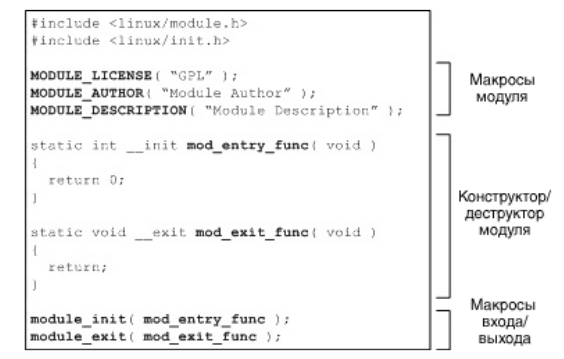
\includegraphics[,scale=0.7]{./img/1.png}
		\caption{Пример загружаемого модуля ядра.}  
		\label{img:1}
\end{figure}
\subsection{Пространство пользователя и пространство ядра}
Модули работают в пространстве ядра, в то время как приложения работают в пользовательском пространстве. 

На практике ролью операционной системы является обеспечение программ надёжным доступом к аппаратной части компьютера. Кроме того, операционная система должна обеспечивать независимую работу программ и защиту от несанкционированного доступа к ресурсам. Решение этих нетривиальных задач становится возможным, только если процессор обеспечивает защиту системного программного обеспечения от прикладных программ.

Каждый современный процессор позволяет реализовать такое поведение. Выбранный подход заключается в обеспечении разных режимов работы (или уровней) в самом центральном процессоре. Уровни играют разные роли инекоторые операции на более низких уровнях не допускаются; программный код может переключить один уровень на другой только ограниченным числом способов. Unix системы разработаны для использования этой аппаратной функции с помощью двух таких уровней. Все современные процессоры имеют не менее двух уровней защиты, а некоторые, например семейство x86, имеют больше уровней; когда существует несколько уровней, используются самый высокий и самый низкий уровни. Под Unix ядро выполняется на самом высоком уровне (также называемым режимом супервизора), где разрешено всё, а приложения выполняются на самом низком уровне (так называемом пользовательском режиме), в котором процессор регулирует прямой доступ к оборудованию и несанкционированный доступ к памяти. Unix выполняет переход из пользовательского пространства в пространство ядра, когда приложение делает системный вызов или приостанавливается аппаратным прерыванием. Код ядра, выполняя системный вызов, работает в контексте процесса - он действует от имени вызывающего процесса и в состоянии получить данные в адресном пространстве процесса. Код, который обрабатывает прерывания, с другой стороны, является асинхронным по отношению к процессам и не связан с каким-либо определённым процессом. 

Ролью модуля является расширение функциональности ядра; код модулей выполняется в пространстве ядра. Обычно драйвер выполняет обе задачи, изложенные ранее: некоторые функции в модуле выполняются как часть системных вызовов, а некоторые из них отвечают за обработку прерываний.

\subsection{Анализ аудио-подсистем}
\subsubsection{Open Sound System}

Open Sound System (OSS) — унифицированный драйвер для звуковых карт и других звуковых устройств в различных UNIX-подобных операционных системах.

OSS основан на Linux Sound Driver и в настоящее время работает на большом числе платформ: Linux, FreeBSD, OpenSolaris и т. д. \cite{3} /dev/dsp и /dev/audio — основные файлы устройств для цифровых приложений. Любые данные, записанные в эти файлы, воспроизводятся на DAC/PCM/DSP устройстве звуковой карты. Чтение из этих файлов возвращает звуковые данные, записанные с текущего входного источника (по умолчанию это Микрофонный вход).

При чтении из /dev/dsp мы получаем несжатый аудиопоток с микрофона компьютера через вход звуковой карты.

\subsubsection{ALSA}
ALSA (англ. Advanced Linux Sound Architecture, Продвинутая звуковая архитектура Linux) — архитектура звуковых драйверов, а также широкий их набор для операционной системы Linux, призванный сменить Open Sound System (OSS). ALSA тесно связана с ядром Linux\cite{4}. Архитектуру звуковой подсистемы Linux показан на рисунке \ref{img:2}.
\captionsetup{justification=centering,singlelinecheck=off}
\begin{figure}[h!]
	\centering
		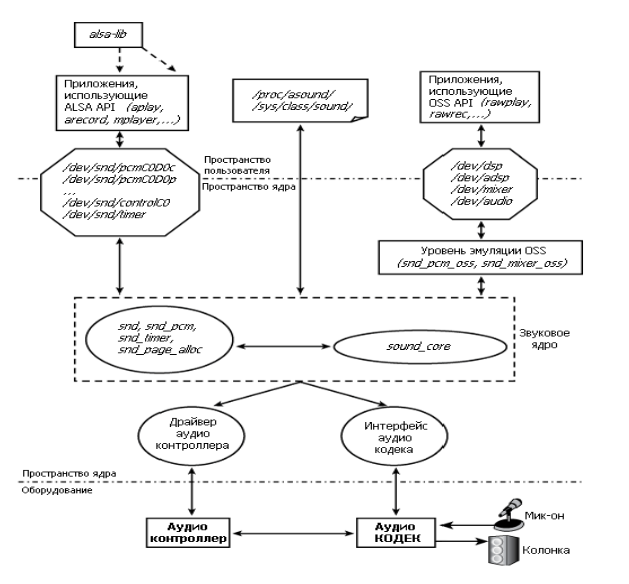
\includegraphics[,scale=0.7]{./img/2.png}
		\caption{Пример загружаемого модуля ядра.}  
		\label{img:2}
\end{figure}

Основными частями подсистемы являются:

а) Звуковое ядро, которое является базовым кодом, состоящим из процедур и структур, доступных другим компонентам звукового уровня Linux. Как и уровни ядра, принадлежащие другим драйверным подсистемам, звуковое ядро обеспечивает уровень косвенности, что делает каждый компонент в звуковой подсистеме не зависящим от других. Ядро играет важную роль в экспорте API ALSA вышележащим приложениям. Узлами /dev/snd/*, показанными на Рисунке 1, которые создаются и управляются из ядром ALSA, являются: /dev/snd/controlC0 - узел управления (используемый в приложениях для управления уровнем громкости и тому подобному), /dev/snd/pcmC0D0p - устройство воспроизведения (p в конце имени устройства означает playback, воспроизведение), и /dev/snd/pcmC0D0c - записывающее устройство (c в конце имени устройства означает capture, захват). В этих именах устройств целое число после C является номером карты, а после D - номером устройства. ALSA драйвер для карты, которая имеет голосовой кодек для телефонии и стерео кодек для музыки, может экспортировать /dev/snd/pcmC0D0p для чтения аудио потоков, предназначенный для первого, и /dev/snd/pcmC0D1p для качественного музыкального канала для последнего;

б) Драйверы аудио контроллера зависят от оборудования контроллера. Например, для управления аудио контроллером, находящимся в Южном мосте Intel ICH, используется драйвер snd\_intel8x0; 

в) Интерфейсы аудиокодеков, которые помогают взаимодействию между контроллерами и кодеками. Для кодеков AC’97 используйте snd\_ac97\_codec и модули ac97\_bus;

г) Уровень эмуляции OSS, который выступает в качестве посредника между приложениями, использующими OSS, и ядром с поддерживающим ALSA. Этот уровень экспортирует узлы /dev, изображающие поддержку уровня OSS в ядре версии 2.4. Эти узлы, такие как /dev/dsp, /dev/adsp и /dev/mixer, позволяют приложениям OSS работать поверх ALSA без изменений. Узел OSS /dev/dsp связан с узлами ALSA /dev/snd/pcmC0D0*, /dev/adsp соответствует /dev/snd/pcmC0D1*, а /dev/mixer связан с /dev/snd/controlC0;

д) Интерфейс procfs and sysfs для доступа к информации через /proc/asound/ и /sys/class/sound/;

е) Библиотека ALSA пользовательского пространства, alsa-lib, которая предоставляет объект libasound.so. Эта библиотека упрощает работу программиста приложения ALSA, предлагая несколько готовых процедур для доступа к драйверам ALSA;

ж) Пакет alsa-utils, который включает в себя такие утилиты, как alsamixer, amixer, alsactl и aplay. alsamixer или mixer используются для изменения громкости звуковых сигналов, таких как линейный вход, линейный выход или микрофон, а alsactl - для управления параметрами драйверов ALSA. aplay используется для воспроизведения звука через ALSA.

\subsection{Анализ реализации отложенных действии}

Для высокоскоростных операций с потоками ядро Linux предлагает тасклеты и очереди работ. С помощью тасклетов и очередей работ реализуются функции отложенного исполнения, что заменяет старый механизм использования нижних половин в драйверах.

\subsubsection{Тасклеты}

Тасклеты являются структурами отложенного исполнения, которые вы можете запланировать на запуск позже в виде зарегистрированных функций. Верхняя половина (обработчик прерываний) выполняет небольшой объем работ, а затем планирует тасклеты, которые будут выполнены позже в нижней половине.

При создании функции тасклета используются соответствующие данные (my\_tasklet\_function и my\_tasklet\_data), который затем используется при объявлении нового тасклета с помощью макроса DECLARE\_TASKLET. Когда модуль вставляется, то планируется исполнение тасклета, что делает его исполняемым в определенный момент в будущем. Когда модуль выгружается, вызывается функция tasklet\_kill для того, чтобы изъять тасклет из состояния запланированного исполнения.

\subsubsection{Очереди работ}
Вместо того, чтобы предлагать однократную схему отложенного исполнения, как в случае с тасклетами, очереди работ являются обобщенным механизмом отложенного исполнения, в котором функция обработчика, используемая для очереди работ, может "засыпать" (что невозможно в модели тасклетов). Очереди работ могут иметь более высокую латентность, чем тасклеты, но они имеют более богатое API для отложенного исполнения работ.

В очередях работ предлагается обобщенный механизм, в котором отсроченная функциональность переносится в механизмы выполнения нижних половин. В основе лежит очередь работ (структура workqueue\_struct), который является структурой, в которую помещается данные объект work. Работа (т.е. объект work) представлена структурой work\_struct, в которой идентифицируется работа, исполнение которой откладывается, и функция отложенного исполнения, которая будет при этом использоваться.

Основная структура для очереди работ сама является очередью. Эта структура используется при обработке очередей механизмом верхней половины, где планируются отложенные действия, передаваемые в нижнию половину на последующее исполнение. Очередь работ создается с помощью макроса с именем create\_workqueue, который возвращает ссылку на workqueue\_struct. Вы позже сможете удалить (при необходимости) эту очередь работ с помощью вызова функции destroy\_workqueue.

\subsection{Анализ структуры ядра}
\subsubsection{struct tty\_driver}
Структура tty\_driver используется, чтобы зарегистрировать tty драйвер в ядре tty. Ниже описаны все различные поля в структуре.
\begin{lstlisting}[caption = Описание struct tty\_driver, label = {lst:21}]
struct tty_driver {
	struct kref kref;          // подсчет ссылок.
	struct cdev **cdevs;       // выделенные/зарегистрированные символьные устройства
	struct module *owner;      // Владелец модуля этого драйвера.
	const char *driver_name;   // Имя драйвера, используемое в /proc/tty и sysfs.
	const char *name;          // Имя узла драйвера.
    int	name_base;             // Начальный номер, используемый при создании имени для устройства
	int	major;                 // Старший номер для драйвера.
	int	minor_start;           // Начальный младший номер для драйвера. 
	unsigned int num;          // Количество младших номеров, связанных с драйверов. 
	short type;                // тип драйвера tty
	short subtype;             // подтип драйвера tty
	struct ktermios init_termios;  // termios, который будет первоначально установлен для каждого терминала
	unsigned long flags;       // Флаги драйвера, как описывалось ранее в этой главе.
	struct proc_dir_entry *proc_entry; // Структура записи драйвера в /proc. 
	struct tty_driver *other;  // Указатель на ведомый tty драйвер.

	struct tty_struct **ttys;  
    // массив активных &struct tty_struct, установленный tty_standard_install() 
    
	struct tty_port **ports;   // массив &struct tty_port
	struct ktermios **termios; // хранилище для termios при каждом закрытии TTY для следующего открытия 
	void *driver_state;        // указатель на произвольные данные драйвера 

	const struct tty_operations *ops; 
    // перехватчики драйвера для TTY. Установите их с помощью tty_set_operations().
    
	struct list_head tty_drivers; // используется внутри для связывания tty_drivers вместе 
}
\end{lstlisting}

\subsubsection{struct tty\_operations}

Структура tty\_operations содержит все функции обратного вызова, который могут быть установлены tty драйверами и вызваны ядром tty. Ниже описаны все различные поля в структуре.
\begin{lstlisting}[caption = Описание struct tty\_operations, label = {lst:21}]
struct tty_operations {
    // lookup - Возвращает устройство tty, соответствующее idx, NULL, если он не используется в данный момент, и значение ERR_PTR в случае ошибки.
    struct tty_struct * (*lookup)(struct tty_driver *driver, struct inode *inode, int idx);
    
    // install - Установите новый tty во внутренние таблицы self.
    int  (*install)(struct tty_driver *driver, struct tty_struct *tty);
    
    // remove - Удалить закрытый tty из внутренних таблиц self.
    void (*remove)(struct tty_driver *driver, struct tty_struct *tty);
    
    // open - процедура вызывается при открытии определенного устройства tty.
    int  (*open)(struct tty_struct * tty, struct file * filp);
    
    // close - процедура вызывается, когда определенное @tty устройство закрывается.
    void (*close)(struct tty_struct * tty, struct file * filp);
    
    // shutdown - процедура вызывается при блокировке tty, когда конкретное устройство tty закрывается в последний раз.
    void (*shutdown)(struct tty_struct *tty);
    
    // cleanup - процедура вызывается асинхронно, когда конкретное устройство tty закрывается в последний раз, освобождая ресурсы.
    void (*cleanup)(struct tty_struct *tty);
    
    // write - процедура вызывается ядром для записи серии (count) символов (buf) в устройство tty.
    int  (*write)(struct tty_struct * tty, const unsigned char *buf, int count);
    
    // put_char - подпрограмма вызывается ядром для записи одного символа ch в устройство tty.
    int  (*put_char)(struct tty_struct *tty, unsigned char ch);
    
    // flush_chars - процедура вызывается ядром после того, как оно записало серию символов в устройство tty с помощью put_char(). 
    void (*flush_chars)(struct tty_struct *tty);
    
    // write_room - процедура возвращает количество символов, которые драйвер tty примет для записи в очередь.
    int  (*write_room)(struct tty_struct *tty);
    
    // chars_in_buffer - процедура возвращает количество символов в частной очереди вывода устройства.
    int  (*chars_in_buffer)(struct tty_struct *tty);
    
    // ioctl -  подпрограмма позволяет драйверу tty реализовывать специфичные для устройства ioctls.
    int  (*ioctl)(struct tty_struct *tty, unsigned int cmd, unsigned long arg);
    
    // compat_ioctl - Реализовать обработку ioctl для 32-битного процесса в 64-битной системе. 
    long (*compat_ioctl)(struct tty_struct *tty, unsigned int cmd, unsigned long arg);
    
    // set_termios - процедура позволяет драйверу @tty уведомлять об изменении настроек termios устройства.
    void (*set_termios)(struct tty_struct *tty, struct ktermios * old);
    
    // stop - процедура уведомляет драйвер tty о том, что он должен прекратить вывод символов на устройство tty
    void (*stop)(struct tty_struct *tty);
    
    // start - процедура уведомляет драйвер tty о том, что он возобновил отправку символов на устройство tty
    void (*start)(struct tty_struct *tty);
    
    // hangup - процедура уведомляет драйвер tty о том, что он должен повесить устройство tty.
    void (*hangup)(struct tty_struct *tty);
    
    // flush_buffer - процедура отбрасывает частный выходной буфер устройства.
    void (*flush_buffer)(struct tty_struct *tty);
    
    // set_ldisc - процедура позволяет драйверу tty уведомляться, когда дисциплина линии устройства изменяется.
    void (*set_ldisc)(struct tty_struct *tty);
    
    // tiocmget- процедура используется для получения битов состояния модема от драйвера tty
    int (*tiocmget)(struct tty_struct *tty);
    
    // tiocmset - процедура используется для установки битов состояния модема в драйвер tty.
    int (*tiocmset)(struct tty_struct *tty,
            unsigned int set, unsigned int clear);
            
    // resize - ызывается, когда выдается запрос termios, который изменяет запрошенную геометрию терминала на ws.
    int (*resize)(struct tty_struct *tty, struct winsize *ws);
    
    // get_icount - Вызывается, когда устройство tty получает %TIOCGICOUNT ioctl.
    int (*get_icount)(struct tty_struct *tty,
                struct serial_icounter_struct *icount);
};
\end{lstlisting}
\subsubsection{struct tty\_port}
Структура tty\_port — содержит все информация об уровне порта. Ниже описаны все различные поля в структуре.
\begin{lstlisting}
struct tty_port {
    struct tty_bufhead buf; // буфер для этого порта, заблокирован внутри
    struct tty_struct *tty; 
    // обратный указатель на &struct tty_struct, действителен только в том случае, если tty открыт.
    
    struct tty_struct *itty;// внутренний обратный указатель на &struct tty_struct.
    const struct tty_port_operations *ops; // операции tty-порта, см. struct tty_port_operations 
    const struct tty_port_client_operations *client_ops; // клиентские операции tty-порта
    spinlock_t lock;        // защита блокировки tty 
    int blocked_open;       // количество процессов, ожидающих открытия в tty_port_block_til_ready() 
    int	count;              // счетчик использования 
    
    wait_queue_head_t open_wait; // открытая очередь ожидающих
    wait_queue_head_t delta_msr_wait; // очередь изменения статуса модема
    
    unsigned long flags;    // пользовательские флаги TTY
    unsigned long iflags;   // внутренние флаги
    unsigned char console:1; // если установлено, порт является консольным 
    struct mutex mutex;     // блокировка для открытия, выключения и другие операции с портом 
};
\end{lstlisting}

\subsubsection{struct tty\_struct}
Структура tty\_struct — состояние, связанное с tty при открытом. Ниже описаны все различные поля в структуре.
\begin{lstlisting}
struct tty_struct {
    struct kref kref;       // подсчет ссылок
    int index;              // индекс этого tty
    struct device *dev;     // устройство класса или %NULL
    struct tty_driver *driver;  // struct tty_driver, управляющий этим tty
    struct tty_port *port;  // постоянное хранилище для этого устройства
    const struct tty_operations *ops;   // struct tty_operations для этого tty
    
    struct tty_ldisc *ldisc;    // текущая дисциплина линии для этого tty
    struct ld_semaphore ldisc_sem; // защищает изменения дисциплины линии (ldisc)
    
    struct mutex atomic_write_lock; // защищает от одновременной записи, т.е. блокировок
    struct mutex legacy_mutex;      // остатки истории 
    char name[64];          // имя tty, созданное tty_line_name() 
    unsigned long flags;    // побитовое ИЛИ
    int count;      
    // количество открытых процессов, достижение нуля отменяет всю работу для этого tty и также удаляет kref
    
    unsigned int receive_room;  
    // байты, разрешенные для передачи в @ldisc без каких-либо изменений потерял 
}
\end{lstlisting}
\subsection*{Вывод}
В данной работе для получения потока байтов от микрофонного разъема будем использовать API, предоставляемые ALSA. Для реализации отложенных действии будем использовать тасклет.